%	====================
% 		  Preamble
%	====================

\documentclass[a4paper, 11pt, letterpaper]{article}

% Import packages
\usepackage[a4paper, bottom = 1.1in,left = 1in,right = 1in,top = 1.1in]{geometry}
\usepackage{charter}
\usepackage{breqn}
\usepackage{enumitem}
\usepackage{amsmath,amsthm,mathtools,amsfonts}

% Add new commands


%	====================
% 	 Start the Document
%	====================

%opening
\title{Bug Algorithms for Motion Planning}
\author{SC627 Assignment 1, Dhananjay Tiwari, 170020019}

\begin{document}

\maketitle

The report describes the implementation of basic motion planning using Bug algorithms for mobile robots moving in a 2D plane. The task of a robot is to move from a start point to an end point in the $x-y$ plane, in the presence of obstacles. Currently, the obstacles are in the form of polygons and the robot is assumed to detect the obstacles, its current position, and position of the goal.

Three types of Bug algorithms are implemented - \textit{bug\_base}, \textit{bug0} and \textit{bug1}. The \textit{bug\_base} is based on principle that the robot keeps moving in the direction of the goal until it reaches there, but it can not move around the obstacles. Thus, \textit{bug\_base} can only succeed if there is no obstacle between the start and the goal. On the other hand, \textit{bug0} and \textit{bug1} make the bot cross the obstacles. The \textit{bug0} algorithm allows the bot to move around the obstacles until it can move towards the goal again. The \textit{bug1} algorithm makes the bot move around obstacles and leave them at points which are nearest to the goal. At every instant, the bot moves with a given step-size, which also determines the resolution of displacement of the bot. It reaches the goal once the distance between its position and the goal is less than the step-size.  

The algorithms are implemented on ROS-Gazebo platform on a turtlebot3. All the results are currently in the form of plots generated in the python files. In the submission folder, there are total six python files - \textit{helper.py}, \textit{testFunctions.py}, \textit{bug\_base.py}, \textit{bug0.py}, \textit{bug1.py} and \textit{move\_xy\_server.py}, one input file - \textit{input.txt} and three output files - \textit{output\_base.txt}, \textit{output\_0.txt}. and \textit{output\_1.txt}. All the geometrical functions, to find line and segment through two points, distance between points and segments, points and obstacles (polygons) and the tangent vector along the polygons at given points are computed in \textit{helper.py}. The algorithm loops are written in \textit{bug\_base.py}, \textit{bug0.py} and \textit{bug1.py} repsectively. These files also communicate with the \textit{move\_xy\_server.py} to reflect the motion of turtlebot3 in ROS-Gazebo.

\subsection{bug\_base}

Figures \ref{fig:bugbase} shows the path followed by the bot for \textit{bug\_base} algorithm. The start point is $\left[0,0\right]^T$, the goal is $\left[5,3\right]^T$ and the step size is $0.1$ displacement units.

At every instant, the algorithm computes the direction of the goal from its current location. Further, it also determines the distance from all the obstacles and if there is any obstacle or not in between. The distance from the obstacles is computed by \textit{computeDistancePointToPolygon} function in \textit{helper.py}. For each obstacle, the \textit{computeDistancePointToPolygon} function determines the distance from each side of the polygon-shaped obstacle. The output of \textit{computeDistancePointToPolygon} includes the minimum distance and the point of closest distance on the obstacle. The previous output comes from the function \textit{computeDistancePointToSegment}, which outputs the point of minimum distance on the segment and the information if the point of closest distance is inside the segment or outside the segment. The closest point is one of the end-points of the segment if the projection lies outside the segment, depending on the location of the projection. Thus, the closest point can be one of the vertices of the polygon or a point on one of its sides.

\begin{figure}
	\centering
	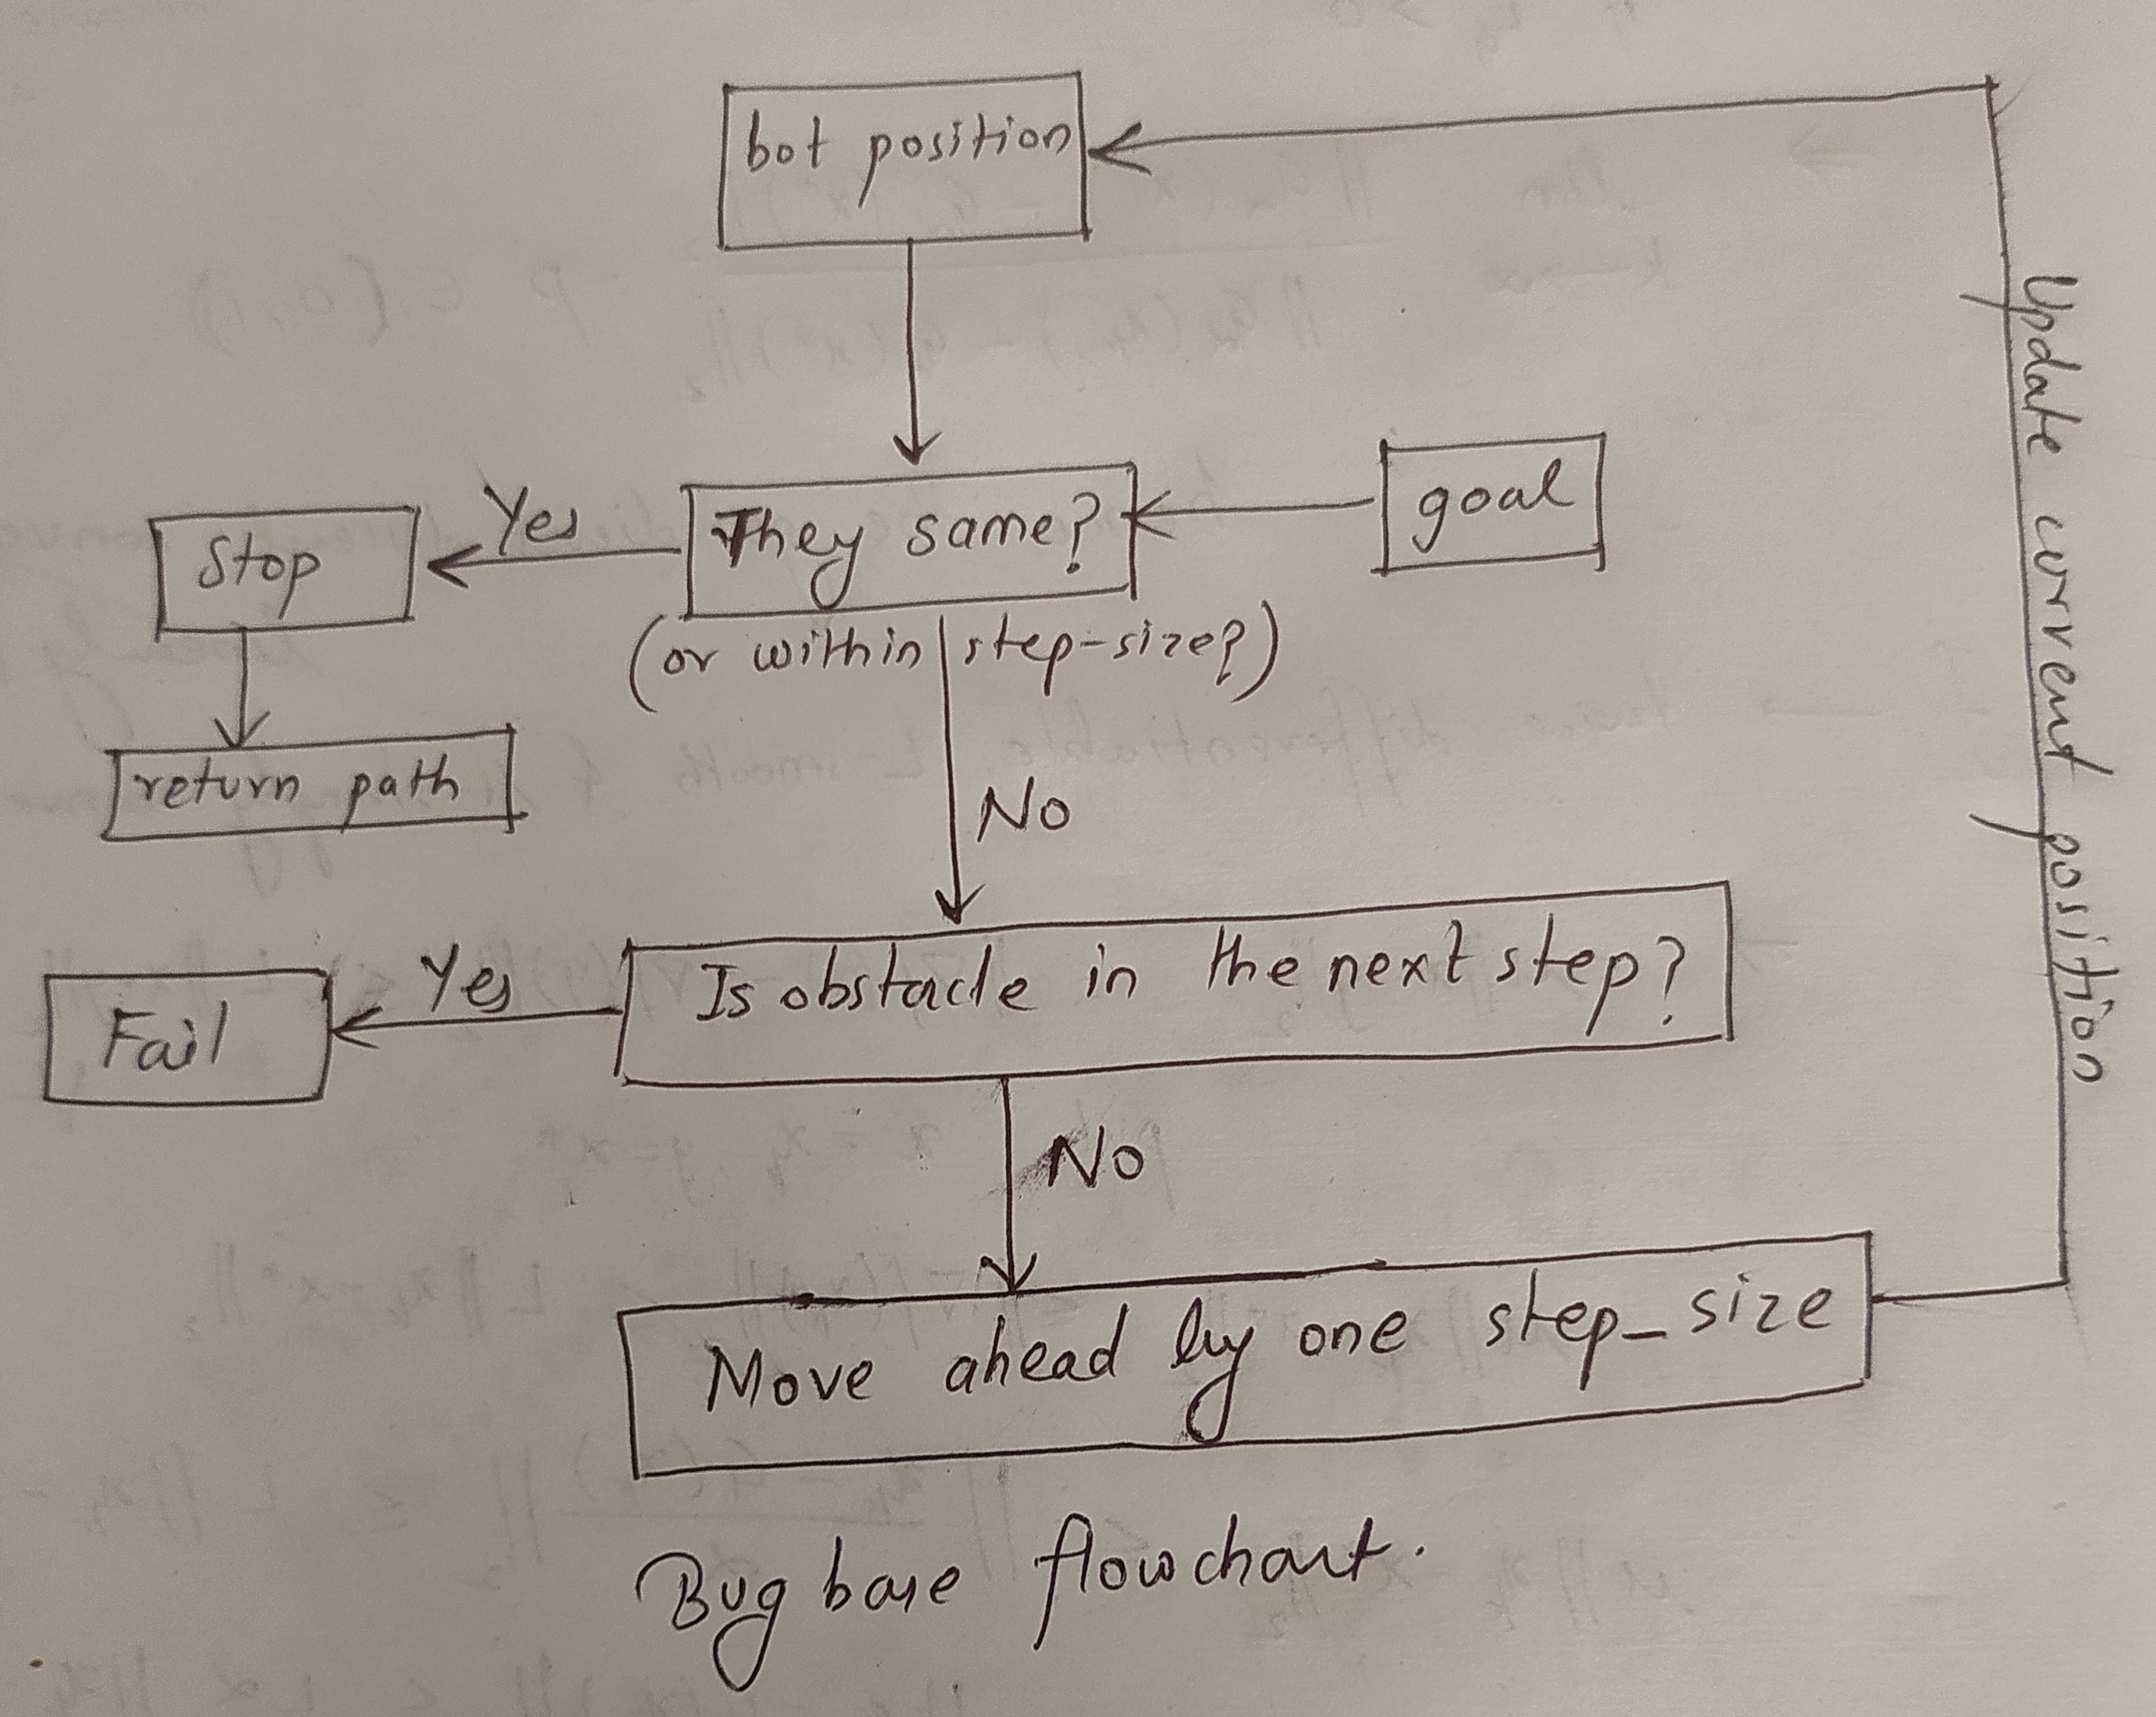
\includegraphics[scale = 0.08]{plots/flowBugBase.jpg}
	\caption{\footnotesize{Flowchart of the bugbase algorithm}}
	\label{fig:flowBugBase}
\end{figure}

If the minimum distance from the obstacle is less than the step size then bot cannot move ahead. However, it is also important to know if the obstacle lies along the direction of the bot. The information can be determined by checking the angle between a vector pointing towards the goal and a vector pointing towards the point of closest distance on the obstacle. The initial point of both the vectors is the current position of the bot. If the angle is less than $90^0$ then the bot will encounter the obstacle, but if the angle is more than or equal to $90^0$ then bot can move towards the goal. The scenario is shown in the figure \ref{fig:obstacledirection}

\begin{figure}
	\centering
	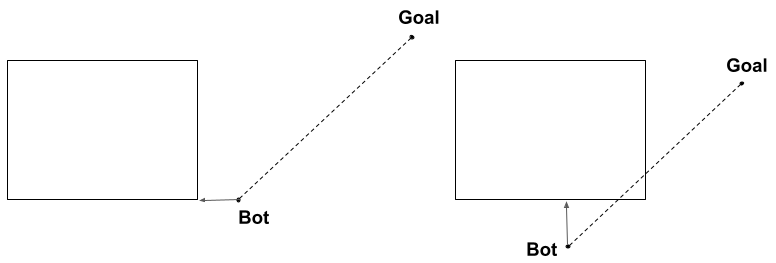
\includegraphics[scale = 0.4]{obstacleDirection.png}
	\caption{\footnotesize{Direction of the obstacle with respect to the bot}}
	\label{fig:obstacledirection}
\end{figure}

\begin{figure}[tbhp!]
	\centering
	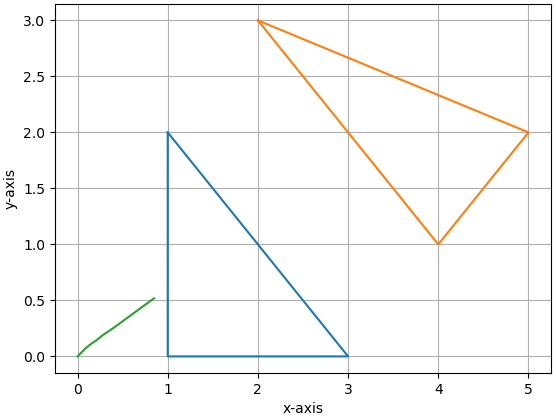
\includegraphics[scale = 0.5]{plots/bugBasePath.png}
	\caption{\footnotesize{Path followed by the bot (green) using \textit{bug\_base} algorithm}}
	\label{fig:bugbase}
\end{figure}


\subsection{bug0}
The path followed by the bot is showed in the figure \ref{fig:bug0}.
The same functions \textit{computeDistancePointToPolygon} and \textit{computeDistancePointToSegment} are used for \textit{bug0} and \textit{bug1} as well. Moreover, they also use the function \textit{computeTangentToPolygon} that determines the direction of motion when the bot enounters the obstacle boundary. Hence, either the bot moves in the tangent vector direction or the in the direction of the goal. The \textit{bug0} algorithm traverses the obstacle boundary until bot can again move towards the goal. This is done by imposing the condition that the bot moves along the obstacle boundary until the distance between obstacle and the bot is more than the step size or the left scenario in figure \ref{fig:obstacledirection} is satisfied. Note that, in figure, no other obstacles are shown along the line, that does not mean bot cannot move if any obstacle falls in between. The bot only needs to know the direction between goal and the current position to move ahead.

\begin{figure}[tbhp!]
	\centering
	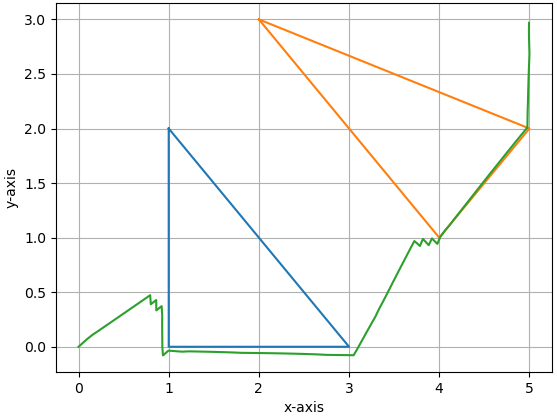
\includegraphics[scale = 0.5]{plots/bug0Path.png}
	\caption{\footnotesize{Path followed by the bot (green) using \textit{bug1} algorithm}}
	\label{fig:bug0}
\end{figure}


\subsection{bug1}

The path followed by the bot is shown in the figure \ref{fig:bug1}. As soon the bot hits its nearest obstacle, the \textit{bug1} algorithm makes it traverse the full obstacle boundary to find a point on the boundary which is at minimum distance from the goal. As soon as the bot hits the obstacle (which is determined by the conditions described in the previous section), it stores the \textit{hit-point} and starts moving in the tangent vector direction. While traversing, the bot keeps storing the points of closest distance, and their distance from the goal until the bot reaches the \textit{hit-point} again. Using the in-built functions \textit{min()} and \textit{numpy.argmin()}, the closest point to the goal is determined on the obstacle boundary. It is called the \textit{leave-point} and bot traverses the boundary again until it reaches the \textit{leave-point} to again start moving along the goal.

\begin{figure}[tbhp!]
	\centering
	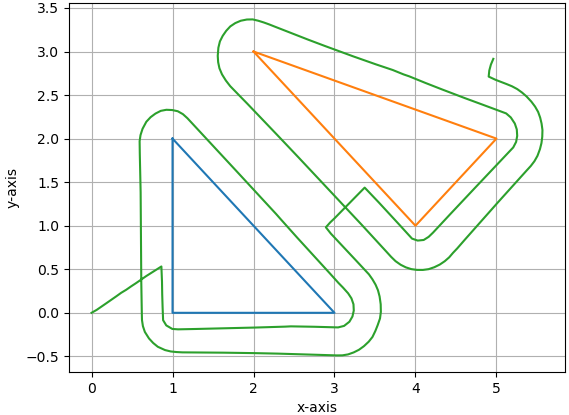
\includegraphics[scale = 0.5]{plots/bug1Path.png}
	\caption{\footnotesize{Path followed by the bot (green) using \textit{bug0} algorithm}}
	\label{fig:bug1}
\end{figure}


\end{document}